\chapter{The human microbiome and atherosclerosis}
\section{Introduction}
In 2010, over half a million deaths in the United States were due to cardiovascular disease \cite{murphy2012deaths}. Atherosclerosis, a chronic disease in which fatty plaques build up in arteries leading to blood clot formation and blockage of the blood stream is a strong contributor to cardiovascular disease. Modifiable risk factors for atherosclerosis include obesity, smoking, physical inactivity, stress, and more. By imaging the carotid artery for atherosclerotic plaques, Spence \cite{spence2012genetics} found that, while the progression of most patients’ atherosclerosis is predicted by their risk factors, some patients present with few factors, and yet their atherosclerosis progresses. Conversely, other patients have many risk factors and their atherosclerosis regresses. Patients on the extreme ends of this spectrum, who exhibit unexplained progressive atherosclerosis or unexplained regressive atherosclerosis will be the focus of this chapter.

Currently the main therapies for atherosclerosis and other cardiovascular disease include a diet low in cholesterol, the cessation of smoking, and the administration of statins to inhibit cholesterol production in the liver. However, in some patients, such as those in this study, these interventions may not be effective. A characterization of the gut and oral microbiome and their effect on cardiovascular disease is necessary to explore atherosclerosis risk factors which are beyond the patient’s explicit control. With this knowledge, the mortality and morbidity of victims of cardiovascular disease may be improved.

\subsection{Atherosclerosis risk}

\begin{figure}[h]
\begin{center}
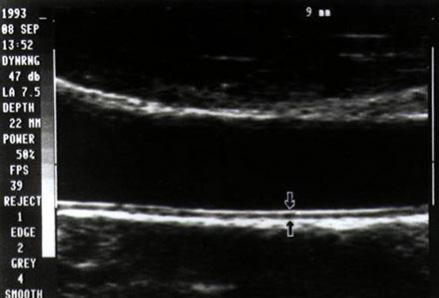
\includegraphics[width=0.7\textwidth]{intima_media_thickness.png}
\caption{\textbf{Carotid Ultrasound showing intima-media thickness}, picture borrowed from Harley Street Cardiologists 2014 London Cardiovascular Clinic. The intima is the innermost layer of the artery bordering the lumen, and the media is the layer just outside that.}
\end{center}
\end{figure}

\begin{figure}[h]
\begin{center}
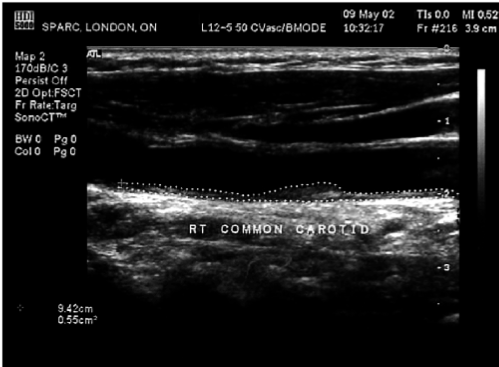
\includegraphics[width=0.7\textwidth]{plaque_area.png}
\caption{\textbf{Carotid Ultrasound showing plaque area measurement}, picture borrowed from Spence \cite{spence2006technology}}
\end{center}
\end{figure}

\begin{figure}[h]
\begin{center}
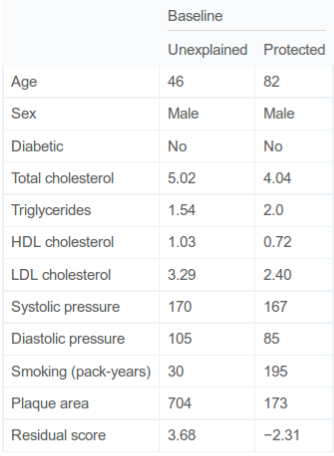
\includegraphics[width=0.5\textwidth]{risk_factors.png}
\caption{\textbf{Risk factors, predicted carotid plaque area, and actual plaque area for two patients.} Two patients’ predicted carotid plaque area based on their risk factors, and their actual plaque area. One patient, a young non-smoker, has a plaque much larger than predicted, and the other patient, an old smoker with a high LDL/HDL ratio has a plaque much smaller than predicted. Both patients are in the top tenth percentile for unexplained atherosclerosis progression or regression. Figure borrowed from Spence \cite{spence2012genetics}.}
\end{center}
\end{figure}

\begin{figure}[h]
\begin{center}
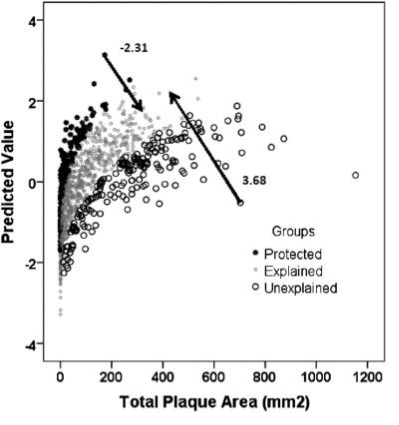
\includegraphics[width=0.7\textwidth]{risk_vs_plaque.png}
\caption{\textbf{Predicted risk vs. total plaque area.} The two arrows represent the residual measures of the two patients in the previous figure. Figure borrowed from Spence \cite{spence2012genetics}.}
\end{center}
\end{figure}

Prior to the advent of measuring atherosclerosis progression directly by carotid ultrasound, pioneered by Dr. J. David Spence, clinicians generally used the measure of intima-media thickness. Tunica intima and tunica media are the two innermost layers of the carotid artery. A greater thickness is due to medial hypertrophy resulting from high blood pressure, and high intima media thickness is correlated with stroke but only weakly predictive of heart attacks \cite{spence2006technology}.

[TO DO: EXPLAIN R SQUARED]

Dr. Spence’s carotid ultrasound technique measures the plaque area. Carotid plaque size appears to have some concordance with both the risk of stroke and myocar-
dial infarction (more so for the latter than the former), while having a much improved correla-
tion with a patient’s risk factors \cite{spence2006technology}. The quartile of carotid plaque size a patient is in correlates with the risk of a stroke or myocardial infarction. Traditional risk factors are able to predict carotid plaque area and volume with R2 = 0.52 (compare with R2 = 0.15 for intima-media thickness), using the regression model developed by Dr. J. D. Spence \cite{spence2012genetics}. The regression model took the following risk factors into account: Age, sex, diabetic status, total cholesterol, triglycerides, HDL cholesterol, LDL cholesterol, systolic pressure, diastolic pressure, lipid or blood pressure medication, and smoking.

Most patients’ actual carotid plaque sizes were relatively close to their predicted carotid plaque sizes, however, some patients presented with plaques much smaller than expected, termed “unexplained atherosclerotic regression” and other patients presented with plaques much larger than expected (“unexplained atherosclerotic progression”). The experiments described in this thesis compare the gut and oral microbiota of the patients with extreme (top 10%) unexplained regression and progression.

\FloatBarrier

\subsection{Metabolic potential of gut microbiota}
A large contributor to a person’s metabolism is the bacteria in their gut. Studies in both mouse and human show that the microorganisms living in each individual \cite{guarner2003gut} can produce hormones \cite{sperandio2003bacteria} and vitamins \cite{burkholder1942synthesis} and even affect brain chemistry \cite{collins2013adoptive}. The following sections will focus on evidence that the gut microbiota contributes to atherosclerosis risk.

\paragraph{Mouse}\mbox{}\\
In mice, it has been found that genetically obese mice \cite{turnbaugh2006obesity} and mice who are obese due to their diet \cite{turnbaugh2008diet} have a lower ratio of members of the phyla Bacteriodetes to members of the phyla Firmicutes, compared to lean mice. Additionally, if gut bacteria from the obese mice are transplanted into lean mice, the lean mice gain weight, despite eating the same diet \cite{turnbaugh2006obesity}. Furthermore, germ-free mice appear to be protected from the effects of diet-induced obesity \cite{backhed2007mechanisms}, and benefit from the increased life span associated with caloric restriction \cite{gordon1966aging}.

\paragraph{Human}\mbox{}\\
Human obese patients also have a lower Bacteriodetes to Firmicutes ratio \cite{turnbaugh2006obesity} in most studies. Certain strains of Firmicutes decreased in proportion as patients dieted, relative to the proportion of the other strains present, increasing the Bacteriodetes : Firmicutes ratio \cite{duncan2008human}. Many metabolites are produced by gut bacteria, including hippurate, phenylacetylglycine, dimethylamine \cite{yap2008metabonomic}, and TMAO \cite{tang2013intestinal}, the latter of which will be examined in depth in the next section.

\paragraph{TMAO: an example of gut bacteria affecting atherosclerosis risk}\mbox{}\\

\begin{figure}[h]
\begin{center}
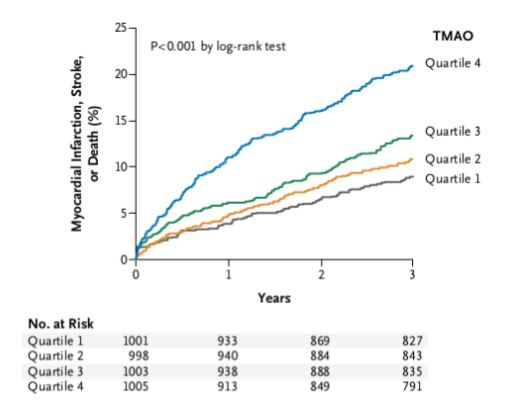
\includegraphics[width=0.7\textwidth]{kaplan_meier.png}
\caption{\textbf{Kaplan-Meier estimates of major adverse cardiovascular events, according to the quartile of TMAO level.} “Data are shown for 4007 participants in the clinical-outcomes study. The P-value is for all comparisons” Figure borrowed from Tang \cite{tang2013intestinal}. Each line of this graph represents data from patients in one of four quartiles for TMAO levels. The risk of myocardial infarction, stroke, or death is more than double for patients who are in the top 25\% for TMAO levels, compared to patients in the bottom quartile.}
\end{center}
\end{figure}

[TO DO: ADD TMAO MECHANISM OF ACTION]

Products of gut metabolism have been shown to affect athlerosclerotic progression. For example, high levels of trimethylamine N-oxide (TMAO) as measured in blood plasma and urine have been associated with higher atherosclerosis risk in humans \cite{tang2013intestinal}. The same association has been reported in mouse models where trimethylamine (TMA) is formed from free choline \cite{al1992exogenous} and phosphatidylcholine \cite{wang2011gut} by bacteria in the mouse gut. TMA that enters the bloodstream from the intestinal tract is later converted to TMAO in the liver. In humans, TMAO has been shown to be produced from L-carnitine, present in red meat \cite{koeth2013intestinal}, and dosing human patients with antibiotics decreased their TMAO levels \cite{tang2013intestinal}.

\FloatBarrier

\subsection{Metabolic potential of mouth microbiota}
There are few studies done on the metabolic contribution of oral microbiota, compared to that of the intestinal microbiota. However, it is known that the mouth can serve as a microbial reservoir for the gut \cite{dal2006oral}.

Many unexpected systemic effects are instigated by, or correlated with, bacteria in the mouth. Plaque containing microbiota may arrive at the bloodstream through ulceration in the gums as a result of gum disease \cite{scannapieco2005systemic} or dental work. Patients have been found to be more at risk for heart attacks and strokes in the 4 weeks immediately following dental treatment \cite{minassian2010invasive}.

Oral microbiota are certainly associated with gum health \cite{marsh1994microbial}, and cardiovascular disease has been correlated with gum infection \cite{beck2005systemic}. Patients with poor gum health are more likely to develop diabetes and diabetic complications \cite{borgnakke2013effect}, rheumatoid arthritis \cite{scher2012periodontal}, and even Alzheimer’s \cite{kamer2008alzheimer}. Pregnant patients with periodontal disease are more likely to experience undesirable pregnancy outcomes \cite{ide2013epidemiology}, such as low birth weight, preterm birth, and pre-eclampsia.

Further proof that oral bacteria may contribute to atherosclerotic plaques is that the combined abundance of Streptococcus and Veillonella appear to be correlated between atherosclerotic plaques and saliva sample taken from the same patient \cite{koren2011human}.

[TO DO: TALK ABOUT THE ORAL MICROBES IN PLAQUE]

\subsection{Bacteria and atherosclerotic plaques}
A 2011 paper by Koren et al. characterized the microbiota present in the atherosclerotic plaques of 15 patients. They found that Pseudomonas luteola, three types of Staphylococcus, three types of Propionibacterineae, and one type of Burkholderia were highly abundant in plaques but not in the oral or gut microbiota. The amount of DNA present in their samples which coded for the 16S ribosomal RNA subunit (indicative of the quantity of bacteria present in the plaque) correlated very strongly with the number of leukocytes in the plaques \cite{koren2011human}. The inflammation response that comes along with increased bacteria in the atherosclerotic plaques plays an important role in plaque growth. Vascular cell adhesion molecule 1 (VCAM-1) binds to these leukocytes, and mice who do not express VCAM-1 exhibit slowed atherosclerotic plaque formation, compared to control mice with the same diet and lipoprotein profiles \cite{cybulsky2001major}. Bacteria-related inflammation status may be a way to explain some of the unexplained atherosclerotic progression or regression.

\subsection{Project proposal}
The main objective of the research I am proposing is to determine the differences in the microbiota of the intestinal tract and oral cavity, between the extreme unexplained progressive atherosclerosis patients and the extreme unexplained regressive atherosclerosis patients. The project will have three different dimensions of analysis. First, a cursory examination of the differential abundance of bacteria between the groups will be done. Then, a metagenomic analysis will follow, to determine the metabolic potential of the microbiome. Lastly, the metabolomics data will connect the differential transcriptomic data to differential metabolite production. All together, these analyses may provide a clearer picture of the processes that produce unexplained progressive and unexplained regressive atherosclerosis.

\section{Methods}
\section{Results}
\section{Discussion}